\documentclass{article}

\usepackage[spanish]{babel}
\usepackage[utf8]{inputenc}
\usepackage[margin=3cm]{geometry}
\usepackage[font=footnotesize,labelfont=bf]{caption}
\usepackage{float}
\usepackage{framed}
\usepackage{color}
\usepackage{wrapfig}\definecolor{shadecolor}{RGB}{224,238,238}
\usepackage{listings}
\usepackage{tikz}
\usepackage{enumitem}
\usepackage{xcolor}

\graphicspath{{images/}}

\title{Trabajo Practico 3: Implementación BIP - Basic Instruction Set Processor}
\author{Perez, Federico\\
        \texttt{perezfederico@unc.edu.ar}
        \and
        Sardoy, Juan Manuel\\
        \texttt{jmsardoy@gmail.com}
        }
\begin{document}

\maketitle
\begin{center}
    
\includegraphics[scale=2]{unc-logo}
\end{center}
\newpage
\section{Descripción del trabajo}

\indent El siguiente trabajo consiste en la implementación práctica de un procesador de propósito educativo
llamado BIP, o Basic Instruction Set Processor. Dicho procesador, tiene la característica de ser muy simple
y de facil entendimiento, lo que facilita el aprendizaje de arquitecturas de computadoras de propósito general.
Es un diseño monociclo, con división de memoria y de canales de datos e instrucciones. En las siguientes secciones
se explicaran los detalles de la arquitectura con mas profundidad. \\
\indent La estructura final de la presentación constará del BIP sintetizado en una FPGA, que se debera comunicar
mediante una interfaz, al modulo UART implementado en el Trabajo Práctico número 2, también sintetizado en dicha FPGA,
que luego mediante un conversor UART/USB, se comunicará con un software corriendo en una computadora personal.
Dentro de la memoria de programa del BIP, deberá existir de forma estática, un programa que ejecute una secuencia de
operaciones matemáticas a elección del implementador. Dicho programa debera iniciar su ejecución, cuando desde la computadora,  se envíe un comando de arranque. Luego, el software en la computadora deberá esperar que el BIP
termine su ejecución y este deberá enviar el resultado por UART, para ser mostrado por pantalla.

\newpage
\section{Arquitectura general}
\indent Como se mencionó anteriormente, se trata de un procesador monociclo,
osea que ejecuta una instrucción por ciclo. Esto trae aparejado el impedimento lógico fundamental de que,
para que una instrucción sea ejecutada , todo el proceso desde que se obtiene la instrucción de la memoria,
hasta su ejecución, debe transcurrir entre dos flancos de clock. Esto límita mucho la velocidad del procesador,
dado que la velocidad del clock esta atada inversamente al tiempo de propagación logica entre los circuitos combinacionales.
Tampoco se puede crear un complejo diseño dado que esto reduciría mas la performance por el mismo motivo.

\begin{figure}[H]
    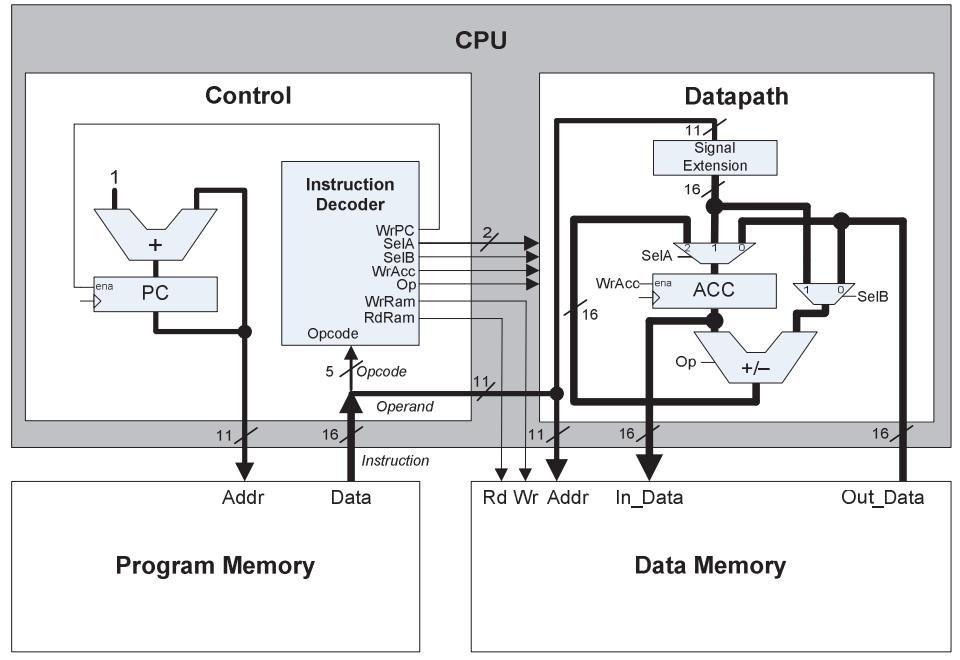
\includegraphics[scale=0.5]{bip_arch}
    \caption{\textit{Diagrama de la arquitectura básica del BIP}}
\end{figure}

Podemos observar claramente los dos bloques principales.
\indent El primero, llamado bloque de \textit{Control}, es el que se encarga de decodificar
la intrucción recibida desde la memoria de programa, y controlar las diferentes señales que operan el resto
del procesador. \\
\indent El segundo, llamado \textit{datapath} o bloque de bus de datos, es el que se conecta con la memoria de datos y ejecuta las operaciones indicadas por el bloque de control. \\ \\

El bloque de control recibe los cinco bits más significativos de cada instruccíon (también llamados \textit{opcode}),
los cuales indican qué instrucción se desea ejecutar.

\begin{figure}[H]
    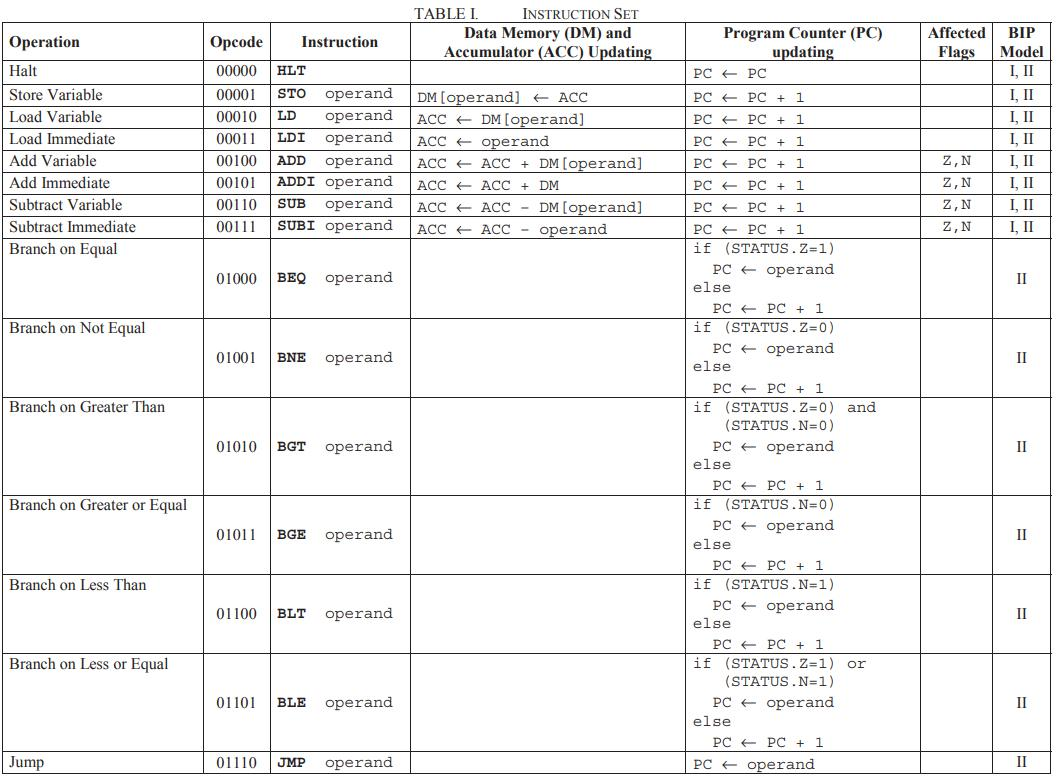
\includegraphics[scale=0.5]{opcodes}
    \caption{\textit{Instrucciones soportadas por el BIP y sus respectivas acciones ejecutadas}}
\end{figure}

Cabe destacar, que dada la consigna del trabajo práctico, no serán implementadas las intrucciones de saltos,
ya sean condicionales o no, con el motivo de hacer mas facil la implementación practica del procesador.
Sin embargo se verá mas adelante, que incluir dichas instrucciones en la implementación es trivial, dado
el diseño modular que se penso para cada parte del sistema.

\newpage
\section{Implementación}

A continuación se detallará la lógica seguida y su implementación en el lenguaje de descripción de hardware Verilog,
para cada módulo del BIP.

\subsection{Memoria de programa}

La memoria de programa es simplemente un arreglo de registros con datos fijos, siendo estos, el programa
\textit{"hardcodeado"} a ejecutar. A continuación, su implementación en Verilog:

\begin{shaded}
\begin{lstlisting}[language=Verilog]
`include "memory_defs.vh"

module ProgramMemory
#(
    parameter ADDRESS_BITS = `ADDRESS_BITS,
    parameter DATA_BITS = `DATA_BITS
)
(
    input clk,
    input rst,
    input wire [ADDRESS_BITS-1:0] i_address,
    output reg [DATA_BITS-1:0] o_data
);

    localparam MEM_SIZE = 2**ADDRESS_BITS;

    reg [DATA_BITS-1:0] mem [0:MEM_SIZE-1];

    `define INSTRUCTION(MNEMONIC, OPCODE) localparam MNEMONIC = OPCODE;
    `include "instructions.vh"

    always@(posedge clk) begin
        if(!rst) begin

            `define                                     \
            DATA_MEMORY(ADDRESS, MNEMONIC, ARGS)        \
                mem[ADDRESS] <= {MNEMONIC, ARGS};

            `include "program.vh"

            //para evitar warning que elimina bits de o_data
            mem[`LAST_ADDRESS] <= {16{1'b1}};
            o_data  <= {16{1'b1}};
        end
        else begin
            o_data <= mem[i_address];
        end
    end

endmodule
\end{lstlisting}
\end{shaded}

Como se ve en el código, también en la definicion de las intrucciones y sus
\textit{opcodes} se utilizo la técnica de X-Macro.

En el archivo \textit{instructions.vh} se observa la definición de todas las instrucciones
definidas por el "standard" del BIP, restando las instrucciones no implementadas, como
se mencionó anteriormente.

\begin{shaded}
\begin{lstlisting}
`ifndef INSTRUCTIONS_VH
`define INSTRUCTIONS_VH

`INSTRUCTION(HLT, 'b00000)
`INSTRUCTION(LD,  'b00010)
`INSTRUCTION(LDI, 'b00011)
`INSTRUCTION(ADD, 'b00100)
`INSTRUCTION(ADDI,'b00101)
`INSTRUCTION(SUB, 'b00110)
`INSTRUCTION(STO, 'b00001)
`INSTRUCTION(SUBI, 'b00111)

`undef INSTRUCTION

`endif
\end{lstlisting}
\end{shaded}

\newpage

Podemos observar que el programa se inserta dentro de la memoria mediante la técnica conocida como \textit{X-Macro}. \\
Esta técnica implia definir una macro para tareas repetitivas, y luego en otro archivo, el cual
será utilizado en el lugar correspondiente, hará uso de dicha macro, listando todos los elementos deseados.
Esto facilita la "programación" y la tarea de debugging, y también reduce la posibilidad de errores,
dado que el mismo tiene una sintáxis mucho mas simple y se encuentra incluido en otro archivo fuente.
Tambien mejora la prolijidad del código, al separar la lógica y datos. \\

Esta tecnica se aplicará en varios lugares a lo largo del proyecto.

El archivo \textit{program.vh} entonces, contendrá el programa propiamente dicho:

\begin{shaded}
\begin{lstlisting}[language=Verilog]
`ifndef PROGRAM_VH
`define PROGRAM_VH

`DATA_MEMORY(0, LDI,  -11'd4)
`DATA_MEMORY(1, STO,   11'd1)
`DATA_MEMORY(2,  LDI,  11'd2)
`DATA_MEMORY(3,  ADD,  11'd1)
`DATA_MEMORY(4,  STO,  11'd2)
`DATA_MEMORY(5,  LDI,  11'd123)
`DATA_MEMORY(6,  ADDI, 11'd7)
`DATA_MEMORY(7,  LD,   11'd2)
`DATA_MEMORY(8,  ADDI, 11'd4)
`DATA_MEMORY(9,  SUBI, 11'd50)
`DATA_MEMORY(10, SUB,  11'd1)
`DATA_MEMORY(11, HLT,  11'd0)

`undef DATA_MEMORY

`endif
\end{lstlisting}
\end{shaded}


El programa realiza una serie de operaciones aritméticas y de transacciones de memoria
(hace uso de todas las instrucciones implementadas), y luego se detiene con la instruccion \textit{HLT o HALT}.

\newpage

\subsection{Memoria de datos}

La memória de datos sigue una lógica muy similar a la de programa, con la salvedad de que la última tiene
un tamaño fijo y vacío. No se cuenta con una memoria con datos iniciales. Todos los datos que se deseen
guardar deben ser guardados en tiempo de ejecución y mediante software. La instrucción para guardar un dato
es \textit{STR o STORE} y para cargarlo es \textit{LD o LDI.}

El código de Verilog para el módulo de la memoria de datos es el siguiente:

\begin{shaded}
\begin{lstlisting}[language=Verilog]
`include "memory_defs.vh"

module DataMemory
#(
    parameter ADDRESS_BITS = `ADDRESS_BITS,
    parameter DATA_BITS = `DATA_BITS
)
(
    input clk,
    input read,
    input write,
    input wire [ADDRESS_BITS-1:0] i_address,
    input wire [DATA_BITS-1:0] i_data,
    output reg [DATA_BITS-1:0] o_data
);

    localparam MEM_SIZE = 2**ADDRESS_BITS;

    reg [DATA_BITS-1:0] mem [0:MEM_SIZE-1];

    always@(negedge clk)
    begin
        if (read)
        begin
            o_data <= mem[i_address];
        end
        else if (write)
        begin
            mem[i_address] <= i_data;
        end
    end
endmodule
\end{lstlisting}
\end{shaded}

\newpage

\subsection{Bloque de Control}

El bloque de control implementa la lógica de decodificación y control de cada una de las instrucciones,
como asi también el Instruction Pointer o IP. El módulo controla todos los elementos, del módulo de datos.
Algunos de los controles que posee son:

\begin{description}[font=$\bullet$~\normalfont\scshape\color{red!50!black}]
\item Habilitar el contador de programa, para que comience a contar.
\item Elegir fuente del registro A y B que van a la ALU. Las fuentes del A pueden ser
memoria, extensor de signo, o realimentación de la ALU misma. Los del B puede ser de
memoria o del extensor de signo. El extensor de signo se explicará en la sección del bloque
datos.
\item Habilitar la escritura del acumulador. El acumulador es un latch que guarda el dato de
entrada con cada ciclo de clock, cuando su señal habilitadora esta en alto.
\item Elegir la operación a efectuar por la ALU. En este caso solamente puede sumar o restar.
\item Leer o escribir RAM. Habilita la RAM de datos para lectura o escritura. Si esta en lectura,
los datos en la dirección de memoria seleccionada por el bus de direcciones, saldran por la salida
de datos. Si esta en escritura, los datos a la salida del acumulador, serán escritos en la dirección
de memoria seleccionada por el bus de direcciones.

\end{description}

\newpage

\subsection{Bloque de bus de datos}


El extensor de signo es un módulo que extiende de un registro
de 11 bits con signo, a uno de 16 bits con signo.
\newpage
\end{document}
